% !TEX program = xelatex
% 그림(ppt_consistency.pdf, brief_summary.pdf, paper_temperature_comparison.pdf)은 이 폴더에서 포함합니다.
\documentclass[10pt,a4paper]{article}

\usepackage{kotex}
\IfFontExistsTF{Malgun Gothic}{
  \setmainhangulfont{Malgun Gothic}
  \setsanshangulfont{Malgun Gothic}
}{
  \setmainhangulfont{Noto Serif CJK KR}
  \setsanshangulfont{Noto Sans CJK KR}
}
\usepackage{amsmath}
\usepackage{booktabs,tabularx,array}
\usepackage{graphicx}
\usepackage{xcolor}
\usepackage{geometry}
\usepackage[hidelinks]{hyperref}
\geometry{top=1.55cm,bottom=1.55cm,left=1.70cm,right=1.70cm}
\setlength{\parindent}{0pt}
\setlength{\parskip}{0.38em}
\setlength{\emergencystretch}{2em}
\renewcommand{\arraystretch}{1.15}

\definecolor{navy}{HTML}{17324D}
\definecolor{teal}{HTML}{0F766E}
\definecolor{orange}{HTML}{C2410C}
\definecolor{pale}{HTML}{EEF6F5}
\definecolor{warn}{HTML}{FFF7ED}
\newcommand{\Status}[1]{\textsf{\footnotesize[#1]}}
\newcommand{\sensunit}{\mathrm{nV\,cm^{-1}\,Hz^{-1/2}}}
\newcommand{\summarybox}[1]{%
  \noindent\colorbox{pale}{%
    \parbox{\dimexpr\textwidth-2\fboxsep\relax}{#1}}}
\newcommand{\warnbox}[1]{%
  \noindent\colorbox{warn}{%
    \parbox{\dimexpr\textwidth-2\fboxsep\relax}{#1}}}

\graphicspath{{./}}
% 본 보고에 사용한 분석 산출값 (2026-07-24 재실행, 38점 온도 격자).
\providecommand{\SlopeOptimumTemperatureC}{43.00}
\providecommand{\SensitivityOptimumTemperatureC}{48.00}
\providecommand{\TotalSensitivityOptimum}{0.967}
\providecommand{\ModelToPPTScaleRoom}{2.06}
\providecommand{\PPTBestPSNLimit}{6.72}
\providecommand{\ModelToPPTScaleOptimum}{7.0}
\providecommand{\GabesOptimumTransmissionPct}{3}
\providecommand{\PaperPSNOptimumC}{33}
\providecommand{\PaperOptimumTransmissionPct}{43}
\providecommand{\RbMeltingC}{39.30}
\providecommand{\ExperimentBestC}{38}
\providecommand{\EITLinewidthMHz}{1.6}
\providecommand{\AbsoluteSensitivityStatus}{PREDICTED}
\providecommand{\ExperimentalInputStatus}{PPT}

\begin{document}

{\color{navy}\LARGE\bfseries Rydberg cell 가열에 따른 RF 감도 변화\par}
\vspace{2pt}
{\large 예비 시뮬레이션 및 주경민 선배님 실험 대조 보고}

\vspace{0.5em}
\begin{tabularx}{\textwidth}{>{\bfseries}p{2.7cm}X}
보고 대상 & 주경민 선배님, ``cell heating 이후 RF sensitivity 변화양상 확인'' (2026-07-15)\\
기준 논문 & G.\ Ju \textit{et al.}, ``Photon shot-noise-limited Rydberg-EIT electrometry,''
           arXiv:2606.04354v1 (선배님 제1저자, 부산대 문한섭 교수님 그룹)\\
시뮬레이션 & GABES --- 박수인이 개발 중인 원자광학 시뮬레이션 코드입니다.
             전체 코드는 \url{https://github.com/Shake2313/fwm-squeezing-app.git}에서 볼 수 있습니다.\\
작성 & 원자광학 시뮬레이션(GABES) 실행 후 AI로 보고서 초안을 작성한 것입니다. 2026년 7월 24일\\
증거 수준 & 발표자료 전사 \Status{PPT}, 선배님 논문 게재값 \Status{REFERENCE},
            전사값에서 유도 \Status{DERIVED}, 시뮬레이션 계산 \Status{PREDICTED},
            미측정 입력 \Status{ASSUMED}/\Status{PENDING}\\
\end{tabularx}

\vspace{0.4em}
\summarybox{%
\textbf{\color{navy}보고 요약}\quad
셀을 가열해 Rb 밀도를 높였을 때 EIT 신호와 RF 최소 검출 전기장이 어떻게 변하는지 확인하여
후속 microwave sensing의 운전 온도를 정하는 시험입니다. 현 시뮬레이션에서 확인된 것은 세 가지입니다.
\textbf{(1)} PPT의 네 온도에서 측정 감도는 그 온도의 PSN limit과 거의 같습니다(비 0.95--1.12).
즉 45/50\,°C에서의 악화는 기술잡음이 더해진 것이 아니라 \textbf{shot-noise floor 자체가 3.7배
나빠진 것}이며, 이는 선배님 시스템이 여전히 near-PSN 영역에서 동작하고 있음과 부합합니다.
\textbf{(2)} PPT 주석의 실제 온도(setpoint 40/45/50 → 38/42.5/44\,°C)를 적용하면
현 시뮬레이션의 slope 최적점 \SlopeOptimumTemperatureC\,°C와 PPT의 EIT 최선명 온도 42.5\,°C가 거의
일치합니다. 광학 응답 경향은 현 시뮬레이션이 맞히고 있습니다.
\textbf{(3)} 가장 중요한 점입니다. 고온에서의 감도 악화는 \textbf{선배님 논문 Fig.\ 5(a)의
온도--PSN 모델이 이미 예측}하는 거동이며(최적 \(\sim\PaperPSNOptimumC\,°C\)), 실측 최적점
\ExperimentBestC\,°C도 그 예측에 가깝습니다. \textbf{오히려 현 시뮬레이션이 감도 최적점을
\SensitivityOptimumTemperatureC\,°C로 너무 높게 내는 것이 확인이 필요한 부분}이며,
이는 현 시뮬레이션이 고온의 투과 광량 고갈(그 지점 투과율 \(\sim\GabesOptimumTransmissionPct\%\))을
과소반영하는 한계로 보입니다.}

\section*{1. 어떤 실험인지, 그리고 기준 논문과의 관계}

발표자료에 담긴 내용은 다음과 같습니다.

\begin{enumerate}
  \setlength{\itemsep}{0.15em}
  \item ceramic heater와 온도 sensor로 vapor cell 가열계를 제작합니다. \Status{PPT}
  \item 상온 및 heater setpoint 40/45/50\,°C에서 EIT 신호를 비교합니다. 45\,°C 설정값에서
        신호가 가장 뚜렷하다고 기록되어 있습니다. \Status{PPT}
  \item 각 조건에서 1\,s 측정 기준 최소 검출 전기장과 PSN limit을 구합니다. PSN 주석에는
        setpoint와 별개로 실제 온도 38 / 42.5 / 44\,°C가 ``??''와 함께 병기되어 있습니다. \Status{PPT}
\end{enumerate}

이 실험은 독립된 heater 검증이 아니라, 선배님 논문(arXiv:2606.04354v1)에서 확립한
\(\mathbf{{}^{85}\mathrm{Rb}}\) 계단형 EIT 원자 초헤테로다인 전기계의 \textbf{운전점 교정} 단계입니다.
그 논문은 상온(\(\sim20\,°C\)) vapor cell에서 \(12.5(8)\,\sensunit\)의 감도(vapor-cell 최고 기록,
PSN 한계 \(11.2\,\sensunit\)에 근접)를 보고했고, \textbf{셀 온도에 따른 PSN 곡선(Fig.\ 5a)까지
이미 제시}하고 있습니다. 본 보고의 온도 대조는 그 곡선을 기준으로 삼습니다.
발표자 계획에도 ``07/16--24 온도에 따른 RF sensitivity 추가 확인''이 있어, 선배님 본인도 이 자료를
확정이 아닌 1차 스캔으로 다루고 계십니다.

\begin{table}[h]
\centering
\small
\caption{PPT 전사값과 그로부터 유도한 비. 감도는 낮을수록 좋습니다. 실제 온도는 PPT의 PSN
주석에 ``??''와 함께 병기된 값입니다. 상온 행은 선배님 논문의 \(\sim20\,°C\) 운전점 수치와 동일합니다.}
\begin{tabular}{lccccl}
\toprule
조건 & 실제 온도 & RF 감도 \((\sensunit)\) & PSN limit & 측정/PSN & 비고\\
\midrule
상온 & \(\sim20\,°C\) & \(12.5(8)\) & 11.2(4) & 1.12 & 선배님 논문 운전점(별도 캠페인)\\
40\,°C setpoint & 38\,°C & \(\mathbf{6.68\pm2.55}\) & 6.72(4) & 0.99 & PPT 기준 최상, \emph{측정 순서상 마지막}\\
45\,°C setpoint & 42.5\,°C & \(17.6\pm2.2\) & 17.6(5) & 1.00 & EIT는 가장 뚜렷함\\
50\,°C setpoint & 44\,°C & \(23.8\pm6.5\) & 25.0(1) & 0.95 & 감도 악화\\
\bottomrule
\end{tabular}
\end{table}

\section*{2. PPT 자체 정합성 진단 \Status{DERIVED}}

모델을 끌어오기 전에, PPT 수치만으로 이미 판별되는 것이 있습니다.

\textbf{측정값이 자기 PSN limit에 붙어 있습니다.} 네 조건 모두 측정/PSN 비가 0.95--1.12로 1 근처입니다.
따라서 45/50\,°C에서의 악화는 detector RIN, 전자단 잡음, 환경 진동 같은 \emph{추가} 기술잡음으로는
설명되지 않습니다. 이 가설군은 이 자료만으로 이미 강하게 배제됩니다.

\textbf{악화한 것은 shot-noise floor 자체입니다.} PSN limit이 6.72 (38\,°C) → 17.6 (42.5\,°C)
→ 25.0 (44\,°C)로 \textbf{3.7배} 나빠집니다. PSN 한계는 검출 광자수와 전기장--전압 변환 기울기로
결정되므로, 원인은 밀도 증가에 따른 \emph{probe 투과량 감소} 또는 \emph{heterodyne 판독 기울기 붕괴}
쪽으로 좁혀집니다. 이는 선배님 논문 Eq.\,(2)의 PSN 공식(감도 \(\propto\) 광자 flux와 기울기의
곱의 역수)이 예측하는 방향과 정확히 같습니다.

\begin{figure}[h]
\centering
\IfFileExists{ppt_consistency.pdf}{%
  
\includegraphics[width=\textwidth]{ppt_consistency}}{%
  \fbox{\parbox{0.9\textwidth}{\centering\vspace{1.2cm}
  그림 파일 \texttt{ppt\_consistency.pdf}을 찾을 수 없습니다.
  \vspace{1.2cm}}}}
\caption{PPT 전사값만 사용한 정합성 진단. 좌: 감도와 PSN limit이 같이 움직이며, x축은 setpoint가
아니라 PPT 주석의 실제 온도입니다. GABES slope 최적점(\SlopeOptimumTemperatureC\,°C)이 EIT 최선명
온도(실제 42.5\,°C)와 겹칩니다. 우: 측정/PSN 비가 모든 조건에서 1 근처입니다.}
\end{figure}

\warnbox{\small\textbf{재현을 위해 확인이 필요한 점 1.}\quad 40\,°C와 50\,°C에서는 측정값이
자기 PSN limit보다 약간 \emph{작습니다}(0.99, 0.95). PSN을 다른 온도·다른 광량 기준으로 계산했거나
대역폭 규약이 달랐을 수 있습니다. 현 시뮬레이션을 실측에 맞추려면 PSN 계산에 쓰인 투과 광량과 ENBW를
원기록에서 확인할 필요가 있습니다.}

\section*{3. 선배님 논문 온도 모델과의 대조 \Status{PREDICTED vs REFERENCE}}

이 대조가 본 보고의 핵심입니다. 선배님 논문 Fig.\ 5(a)는 셀 온도에 대한 PSN 한계 곡선을
제시하며, \textbf{최적점을 \(\sim\PaperPSNOptimumC\,°C\)}로, 그리고 \(\sim39\,°C\) 부근의 증기압
\textbf{불연속}(Rb 고체→액체 상전이)을 보고합니다. 현 시뮬레이션을 38점 온도 격자
(20--55\,°C)로 재실행해 PSN(T)와 투과율(T)을 산출했습니다.

\begin{figure}[h]
\centering
\IfFileExists{paper_temperature_comparison.pdf}{%
  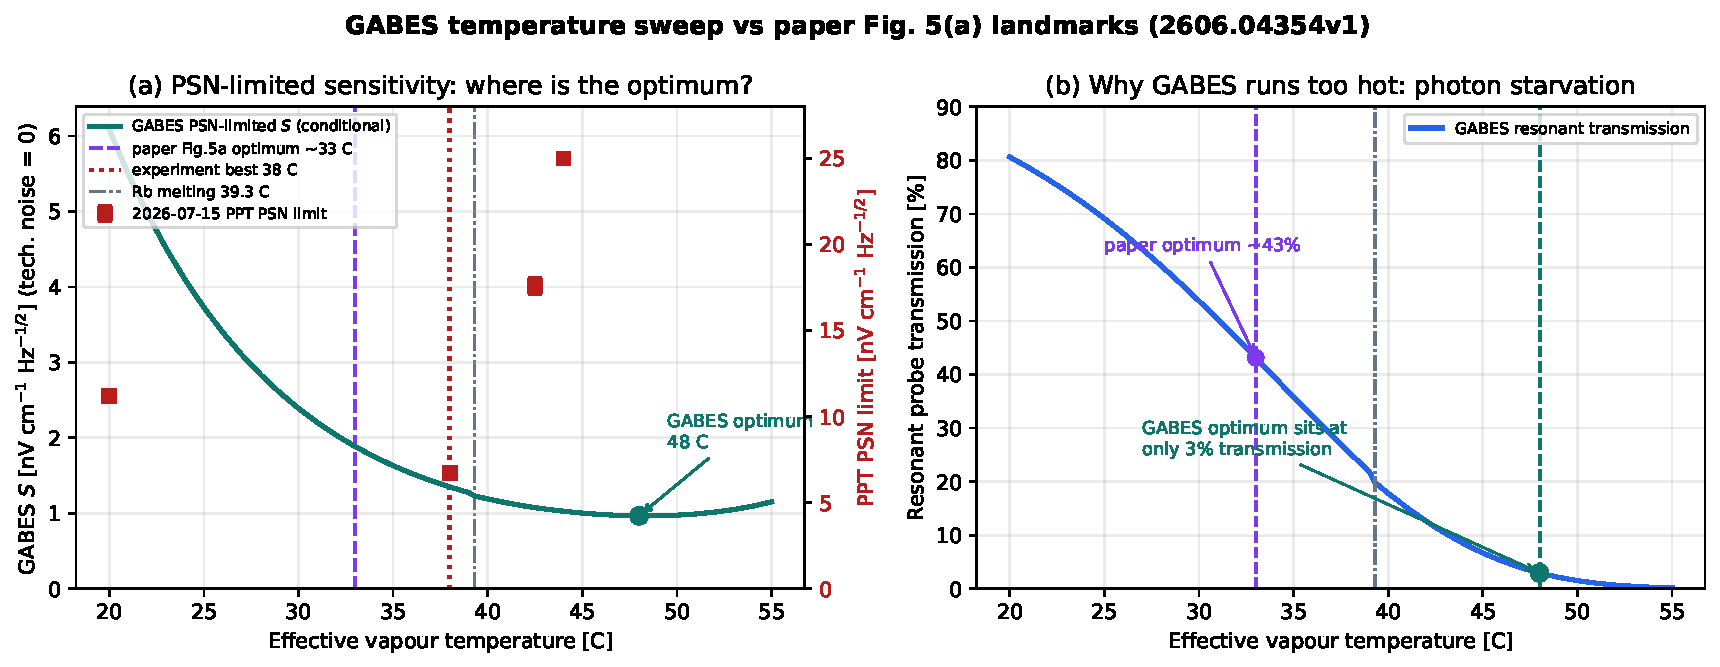
\includegraphics[width=\textwidth]{paper_temperature_comparison}}{%
  \fbox{\parbox{0.9\textwidth}{\centering\vspace{1.0cm}
  그림 파일 \texttt{paper\_temperature\_comparison.pdf}을 찾을 수 없습니다.
  \vspace{1.0cm}}}}
\caption{GABES 온도 스윕과 선배님 논문 Fig.\ 5(a) 랜드마크의 대조. 좌: GABES의 조건부 PSN 감도(청록,
좌축)는 최소가 \SensitivityOptimumTemperatureC\,°C인 반면, 논문 최적(\(\sim\PaperPSNOptimumC\,°C\),
보라 파선)과 실측 최상점(\ExperimentBestC\,°C, 빨강 점선)은 더 낮은 온도에 있습니다. 빨강 사각형은
PPT 전사 PSN(우축, 절대 눈금이 달라 별도 축). 우: 그 원인 — GABES 공진 투과율은
\SensitivityOptimumTemperatureC\,°C에서 이미 \(\sim\GabesOptimumTransmissionPct\%\)까지 떨어져,
그 최적점은 셀이 거의 불투명한 영역에 놓입니다. 회색 일점쇄선은 Rb 융점 \RbMeltingC\,°C.}
\end{figure}

\textbf{경향의 방향은 세 가지가 일치합니다.} 논문 모델(\(\sim\PaperPSNOptimumC\,°C\)), 실측 최상점
(\ExperimentBestC\,°C), 그리고 상온 대비 개선이라는 정성적 그림은 모두 ``상온보다 조금 데우면
좋아지고, 어느 지점을 지나면 다시 나빠진다''를 가리킵니다. 즉 42.5/44\,°C에서의 악화는 정체불명의
이상 현상이 아니라, \textbf{PSN 곡선의 고온 쪽 하강부}로 이미 논문이 설명하는 거동입니다.

\textbf{어긋나는 것은 현 시뮬레이션입니다.} 그 감도 최적점은 \SensitivityOptimumTemperatureC\,°C로,
논문(\(\sim\PaperPSNOptimumC\,°C\))보다 약 15\,°C, 실측(\ExperimentBestC\,°C)보다 약 10\,°C 높습니다.
오른쪽 패널이 이유를 보여줍니다. 현 시뮬레이션은 밀도가 올라갈수록 응답도(responsivity) 이득을 계속
취하다가 \textbf{공진 투과율이 \(\sim\GabesOptimumTransmissionPct\%\)}(광자 고갈)까지 떨어진 뒤에야
최적점을 잡습니다. 반면 논문 최적점(\(\sim\PaperPSNOptimumC\,°C\))은 투과율이 아직
\(\sim\PaperOptimumTransmissionPct\%\)로 건강한 영역입니다. \textbf{현 시뮬레이션이 투과 광량 고갈을
과소반영해 최적점을 너무 고온으로 밀고 있다}는 뜻이며, 이것이 실측의 고온 악화를 재현하지
못하는 직접적 원인으로 보입니다.

\warnbox{\small\textbf{물리 맥락 하나.}\quad 가열 구간 38--50\,°C는 Rb 융점 \RbMeltingC\,°C를
가로지릅니다. 상온·38\,°C는 고체상, 40/45/50\,°C는 액체상 증기압 곡선을 따르므로 밀도--온도 기울기가
융점에서 꺾입니다(우측 패널의 \RbMeltingC\,°C 표시). 선배님 논문도 \(\sim39\,°C\) 불연속을
명시합니다. 현 시뮬레이션은 이 고체/액체 분기를 이미 반영하지만(species.py의 CRC 증기압), 위 최적점
불일치는 융점 처리 때문이 아니라 투과 광량 항의 문제입니다.}

\section*{4. 시뮬레이션 광학/RF 응답 대조}

계산은 \({}^{85}\mathrm{Rb}\) \(5S_{1/2}\!\rightarrow5P_{3/2}\!\rightarrow40D_{5/2}\) EIT와
\(40D_{5/2}\!\rightarrow39F_{7/2}\) RF 결합을 사용했습니다(상태·기하·전력은 모두 선배님 논문 게재값).
각 온도에서 정상상태 OBE spectrum을 구하고, 40-kHz finite-IF weak-SIG 선형 응답, RF dipole,
probe shot noise를 전기장 ASD로 변환했습니다.

\begin{tabularx}{\textwidth}{>{\bfseries}p{3.4cm}X}
논문 게재 입력 & probe 6\,$\mu$W, coupling 30\,mW, beam 0.15\,mm, cell 50\,mm,
  LO Rabi 3.7\,MHz, coupling Rabi 3.0\,MHz, 상태 \(40D_{5/2}\)/\(39F_{7/2}\),
  검출 양자효율 95\,\%, IF 40\,kHz \Status{REFERENCE}\\
조건부 가정 & Doppler off, temperature/density dephasing 0, technical noise 0,
  RF angular factor 1, heater=effective vapor=cold spot, detector path efficiency 0.5 \Status{ASSUMED}\\
결과 상태 & 절대 감도 \Status{\AbsoluteSensitivityStatus}, 실험 입력 \Status{\ExperimentalInputStatus};
  실험값에 맞춘 fitting은 하지 않았습니다\\
\end{tabularx}

이 입력들은 대부분 선배님 논문에 게재된 값이므로 \Status{REFERENCE}로 다룹니다. 따라서 절대 감도의
격차를 선배님 입력의 불확실성 탓으로 볼 근거는 약하며, 격차는 현 시뮬레이션의 근사에서 옵니다.

\begin{figure}[h]
\centering
\IfFileExists{brief_summary.pdf}{%
  
\includegraphics[width=\textwidth]{brief_summary}}{%
  \fbox{\parbox{0.9\textwidth}{\centering\vspace{1.0cm}
  그림 파일 \texttt{brief\_summary.pdf}을 찾을 수 없습니다.
  \vspace{1.0cm}}}}
\caption{GABES 온도 sweep과 PPT 관측의 비교. 회색 점선은 절대 보정 오차를 분리해 온도 경향만
보기 위해 상온 PPT 값에 정규화한 모델입니다.}
\end{figure}

\textbf{광학 응답: 경향이 맞습니다.} 현 시뮬레이션의 spectral slope는 \(\SlopeOptimumTemperatureC\,°C\)에서
최대입니다. PPT의 ``EIT가 가장 뚜렷한'' 조건은 45\,°C setpoint이지만 실제 온도로는 42.5\,°C이므로,
두 값은 0.5\,°C 이내로 겹칩니다. 다만 PPT의 ``뚜렷함''은 contrast/진폭 관찰이고 현 시뮬레이션의 지표는 slope이므로,
이 일치는 정성적 수준으로만 봅니다.

\textbf{RF 감도 절대값: 아직 어긋납니다.} 절대값 격차가 균일하지 않습니다. 상온에서는 실측이 모델
대비 약 \ModelToPPTScaleRoom 배이지만, 최적점 부근에서는 실험 PSN \PPTBestPSNLimit\ 대 모델
\TotalSensitivityOptimum 로 약 \ModelToPPTScaleOptimum 배입니다. \textbf{단일 scale factor로
흡수되지 않습니다.} 3절의 온도 최적점 불일치와 합치면, 잔존 원인은 아래로 좁혀집니다.

\begin{tabularx}{\textwidth}{>{\bfseries\raggedright\arraybackslash}p{4.0cm}X}
\toprule
이 자료로 배제 & 추가 technical noise(RIN, 전자단, 진동) --- 측정/PSN 비가 1 근처\\
\midrule
현 시뮬레이션 쪽 (유력) & 고온 투과 광량 고갈의 과소반영(최적점을 \SensitivityOptimumTemperatureC\,°C로
  과열시킴); Doppler off·dephasing 0으로 인한 EIT 선폭 과소평가(실측 \EITLinewidthMHz\,MHz,
  transit-time 한계)와 그에 따른 slope 과대평가\\
실측 쪽 (확인 필요) & 밀도 의존 collisional dephasing에 의한 slope 붕괴; cold-spot 실패에 따른
  창면 응축·투과량 손실; heater 구조물의 37\,GHz 산란에 의한 LO Rabi 변화\\
공통 (확인 필요) & 실제 vapor 온도와 setpoint의 비선형 관계; Zeeman·MW standing wave의 온도 상관 변화\\
\bottomrule
\end{tabularx}

\section*{5. 판단, 한계 및 다음 측정}

\summarybox{%
\textbf{\color{navy}판단}\quad
현재 자료로 말할 수 있는 것은 \textbf{``40\,°C setpoint(실제 38\,°C)를 유력 후보로 두고 재확인''}까지입니다.
40\,°C가 상온보다 좋아 보이고 이는 선배님 논문 온도 모델(최적 \(\sim\PaperPSNOptimumC\,°C\))과도
같은 방향입니다. 다만 상온 대비 차이는 \(5.8\)에 대해 합성 오차 \(4.4\), 약 1.3$\sigma$이고,
슬라이드 순서상 40\,°C가 마지막 측정이라 시간 드리프트(lock 품질, MW power, 정렬)와 온도 효과가
아직 분리되지 않습니다. \textbf{따라서 ``가열이 감도를 개선한다''는 물리적으로 그럴듯하지만 이
스캔만으로 확립되었다고 말하기는 이릅니다.} 45\,°C는 EIT visibility가 좋은 광학 운전점이지 RF
sensitivity 최적점은 아닙니다. 그리고 현 시뮬레이션의 \(\SensitivityOptimumTemperatureC\,°C\)는
기술잡음 0인 조건부 PSN 기준선이자 \emph{과열된} 최적점이므로, 실험 목표 온도로 인용해서는 안 됩니다.}

\subsection*{권장 재측정 순서}

\begin{enumerate}
  \setlength{\itemsep}{0.22em}
  \item \textbf{측정 순서 무작위화·반복.} 상온을 이번 setup에서 다시 측정해 기준점을 이 캠페인 안으로
        가져오고, 33, 36, 38, 40, 42\,°C를 조밀하게 반복하며 45, 48\,°C를 대조점으로 둡니다.
        논문 최적 \(\sim\PaperPSNOptimumC\,°C\) 부근을 포함하도록 저온 쪽을 넓히면 좋겠습니다.
        가열/냉각 양방향으로 드리프트와 온도 효과를 분리합니다. \emph{07/16--24 계획의 최우선 항목.}
  \item \textbf{투과 광량을 온도마다 기록.} 2·3절의 진단이 맞다면 PSN 악화와 현 시뮬레이션의 최적점 과열은
        모두 투과 probe 광량으로 판별됩니다. DC 투과 전력과 heterodyne slope(V per V/m)를 감도와
        함께 남기면, 실측의 악화 원인과 현 시뮬레이션의 투과 항 오차를 동시에 확인할 수 있습니다.
  \item \textbf{온도장 실측.} heater setpoint 외에 양단 sensor, beam 부근 effective temperature,
        cold-spot 후보 온도를 함께 기록합니다. PPT PSN 주석의 38/42.5/44\,°C가 무엇을 뜻하는지
        원기록에서 확정할 필요가 있습니다.
  \item \textbf{잡음 규약 고정.} raw EIT scan, RF sweep, detector dark trace와 PSD를 저장하고
        RBW, VBW, ENBW, averaging time, peak/RMS convention을 함께 기록합니다.
\end{enumerate}

\subsection*{보고 시 반드시 붙일 한계}

\begin{tabularx}{\textwidth}{>{\bfseries\raggedright\arraybackslash}p{3.35cm}p{2.05cm}X}
\toprule
항목 & 상태 & 의미\\
\midrule
PPT 수치 & \Status{PPT} & raw trace에서 재계산하지 않은 수동 전사값\\
상온 데이터 출처 & \Status{REFERENCE} & 12.5(8)/11.2(4)는 선배님 논문의 \(\sim20\,°C\) 운전점 수치.
  heater 설치 전 다른 캠페인이므로 같은 sweep에 넣을 때 주의\\
측정 순서·드리프트 & \Status{PENDING} & 온도 효과와 시간 드리프트 미분리\\
시뮬레이션 spectrum & \Status{PREDICTED} & reference-anchored 정상상태 OBE 결과\\
절대 RF 감도 & \Status{PREDICTED} & 기술잡음 0인 조건부 PSN 기준; 실험 감도 아님\\
모델 입력 & \Status{REFERENCE} & coupling power, beam waist, cell 길이, LO/coupling Rabi는
  선배님 논문 게재값\\
투과 광량 항 & \Status{PREDICTED} & 고온 최적점을 과열시키는 현 시뮬레이션의 유력 오차원\\
온도장·cold spot & \Status{ASSUMED} & 설정값을 vapor/cold-spot 온도와 동일시\\
Zeeman·RF 공간장 & \Status{PENDING} & 편광, standing wave, 3D field 미포함\\
raw EIT/PSD/log & \Status{PENDING} & 정량 검증과 dephasing/noise fitting에 필요\\
\bottomrule
\end{tabularx}

\subsection*{최종 결론}

현 시뮬레이션은 이 실험의 \textbf{광학 응답 온도 경향}을 이미 맞히고 있고, 이상적 PSN 기준선도 제공합니다.
그리고 선배님 논문 Fig.\ 5(a)의 온도 모델과 실측을 함께 놓고 보면, 고온에서의 감도 악화는 정체불명의
현상이 아니라 \textbf{PSN 곡선의 고온 하강부}로 설명됩니다. 다만 현 시뮬레이션은 감도 최적점을
\(\SensitivityOptimumTemperatureC\,°C\)(투과율 \(\sim\GabesOptimumTransmissionPct\%\))로 과열시켜
그 하강부를 재현하지 못합니다. 따라서 다음 단계는 선배님 실험을 의심하는 것이 아니라, \emph{현 시뮬레이션의
투과 광량 항과 EIT 선폭(\EITLinewidthMHz\,MHz, transit-time 한계)을 실측 투과 로그로 보정하는 것}입니다.
현 단계의 적절한 표현은 ``검증 완료''가 아니라 \textbf{예비 시뮬레이션 및 모델 한계 진단}입니다.
위 raw data와 온도 로그가 확보되면 density-dependent dephasing과 cold-spot density를 순차적으로 식별해
정량 모델로 확장할 수 있습니다.

\vfill
{\footnotesize
\textbf{재현 정보:} 본 보고의 정량값은 발표자료(2026-07-15) 전사 수치와 시뮬레이션 정상상태 OBE 계산
결과를 명확히 구분해 사용했습니다. 3절 그림은 GABES 38점 온도 격자 재실행 결과에 선배님 논문 Fig.\ 5(a)의
\emph{보고된} 랜드마크(최적 \(\sim\PaperPSNOptimumC\,°C\), 융점 \RbMeltingC\,°C)와 PPT 전사 PSN 점을
겹친 것이며, 논문의 곡선 자체를 재구성하지는 않았습니다. 2절 그림은 발표자료 전사 수치만으로 생성했고,
GABES 최적점 주석선 두 개 외에는 모델 값을 쓰지 않았습니다. 원본 발표자료는 수정하지 않았습니다.
분석 재실행일: 2026년 7월 24일.}

\end{document}
